\subsection{Related Standards}
\subsubsection{C++14} The project is programmed in C++ according to the C++14 standard provided by Texas Instruments' ARM compiler. This standard is formally known as ISO/IEC 14882:2014. C++ is a superset of C, and builds upon it by introducing object-oriented programming concepts while maintaining the functional language aspect of C.

\subsubsection{POSIX} The MCU supports threading either through TI-RTOS or POSIX. For this project, POSIX---the Portable Operating System Interface specificed by IEEE 1003.1-2017---defines a shared interface between operating systems and applications. \texttt{pthreads} were used to create different tasks pertaining to management of the charge controller, water solenoid, sensing subsystem, and the HTTP web server.

\subsubsection{802.11} The MCU supports transmission through the IEEE 802.11b/g/n standard of wireless communication. This standard uses the S band of radio frequences and operates at 2.4 GHz. There are 14 accessible channels, each spanning a band width of 22 MHz (pictured in \autoref{wifi_channels}).
\begin{figure}[H]
    \caption{802.11b/g/n channels \cite{Flickenger}}
    \label{wifi_channels}
    \centering
    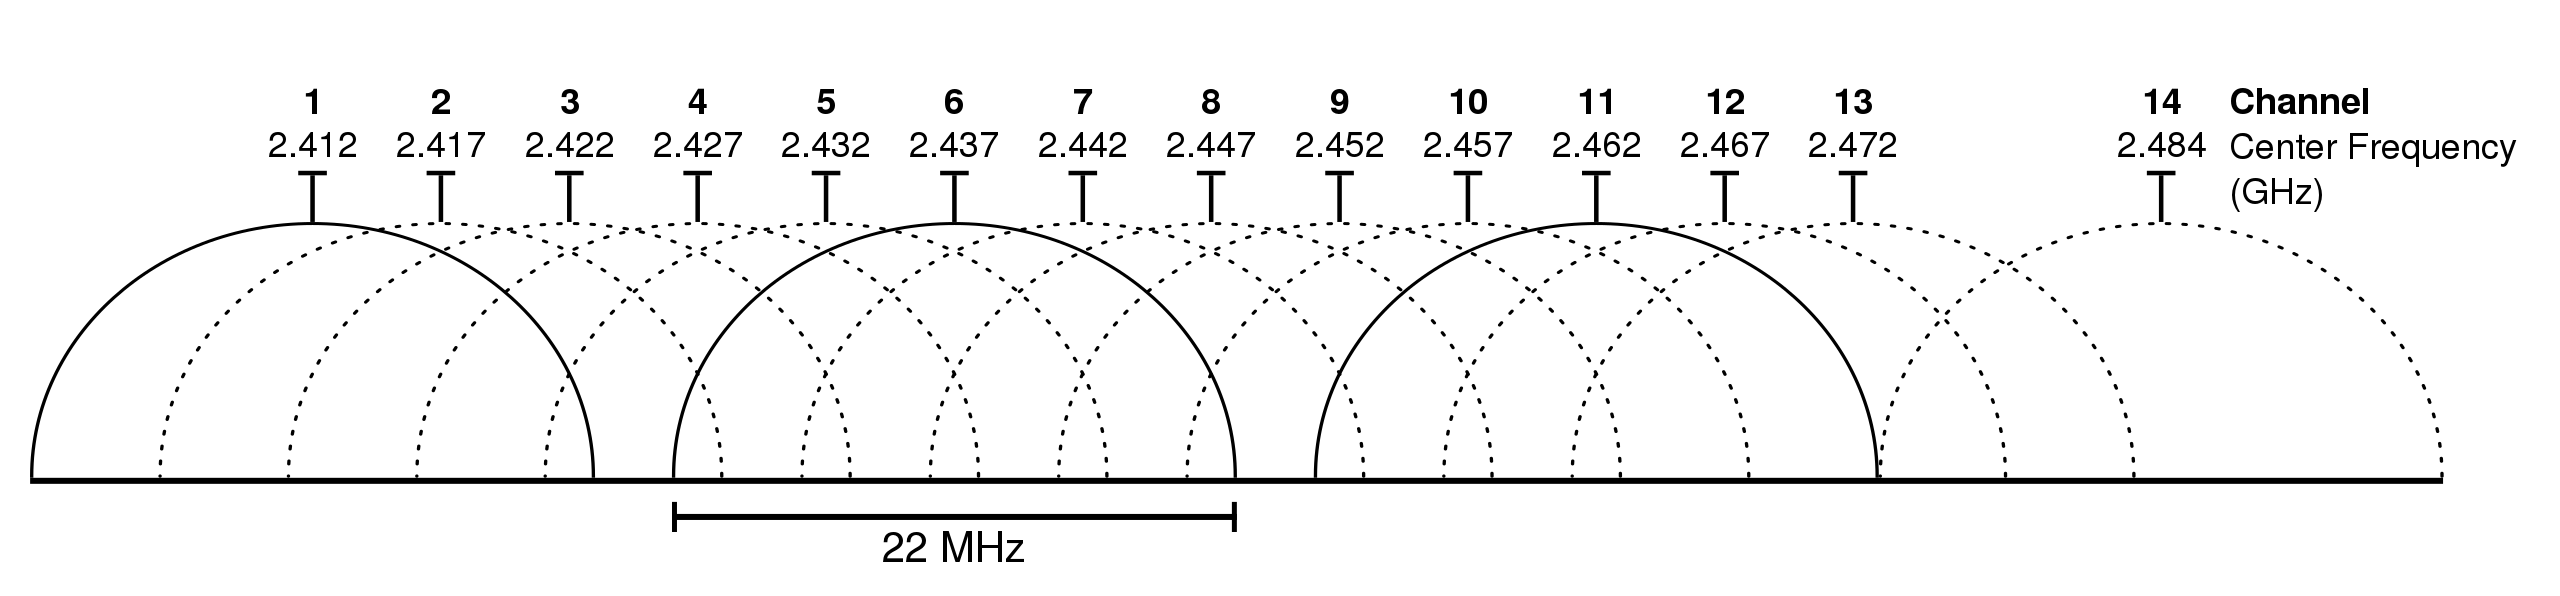
\includegraphics[width=\textwidth]{images/wifi_channels.png}
\end{figure}
These channels specifically reside in an industrial, scientific and medical (ISM) band. This standard also provides datagram frames for the transport layer.

\subsubsection{IPv4} IPv4 is the fourth version of the Internet Protocol, a network layer protocol in use to relay data between devices and across networks. The data relayed, datagrams, are sent between sources and hosts that are identified by 32-bit addresses. This protocol strictly functions to transport the datagram from one device to another, with no end-to-end reliability, flow control, sequencing, or other measures found in other protocols such as TCP. IPv4 provides two distinct features: fragmentation of whole datagrams, and addressing of devices. A standard IPv4 frame is shown in \autoref{ipv4_frame}.
\begin{figure}[H]
    \caption{IPv4 frame \cite{Postel1981}}
    \label{ipv4_frame}
    \centering
    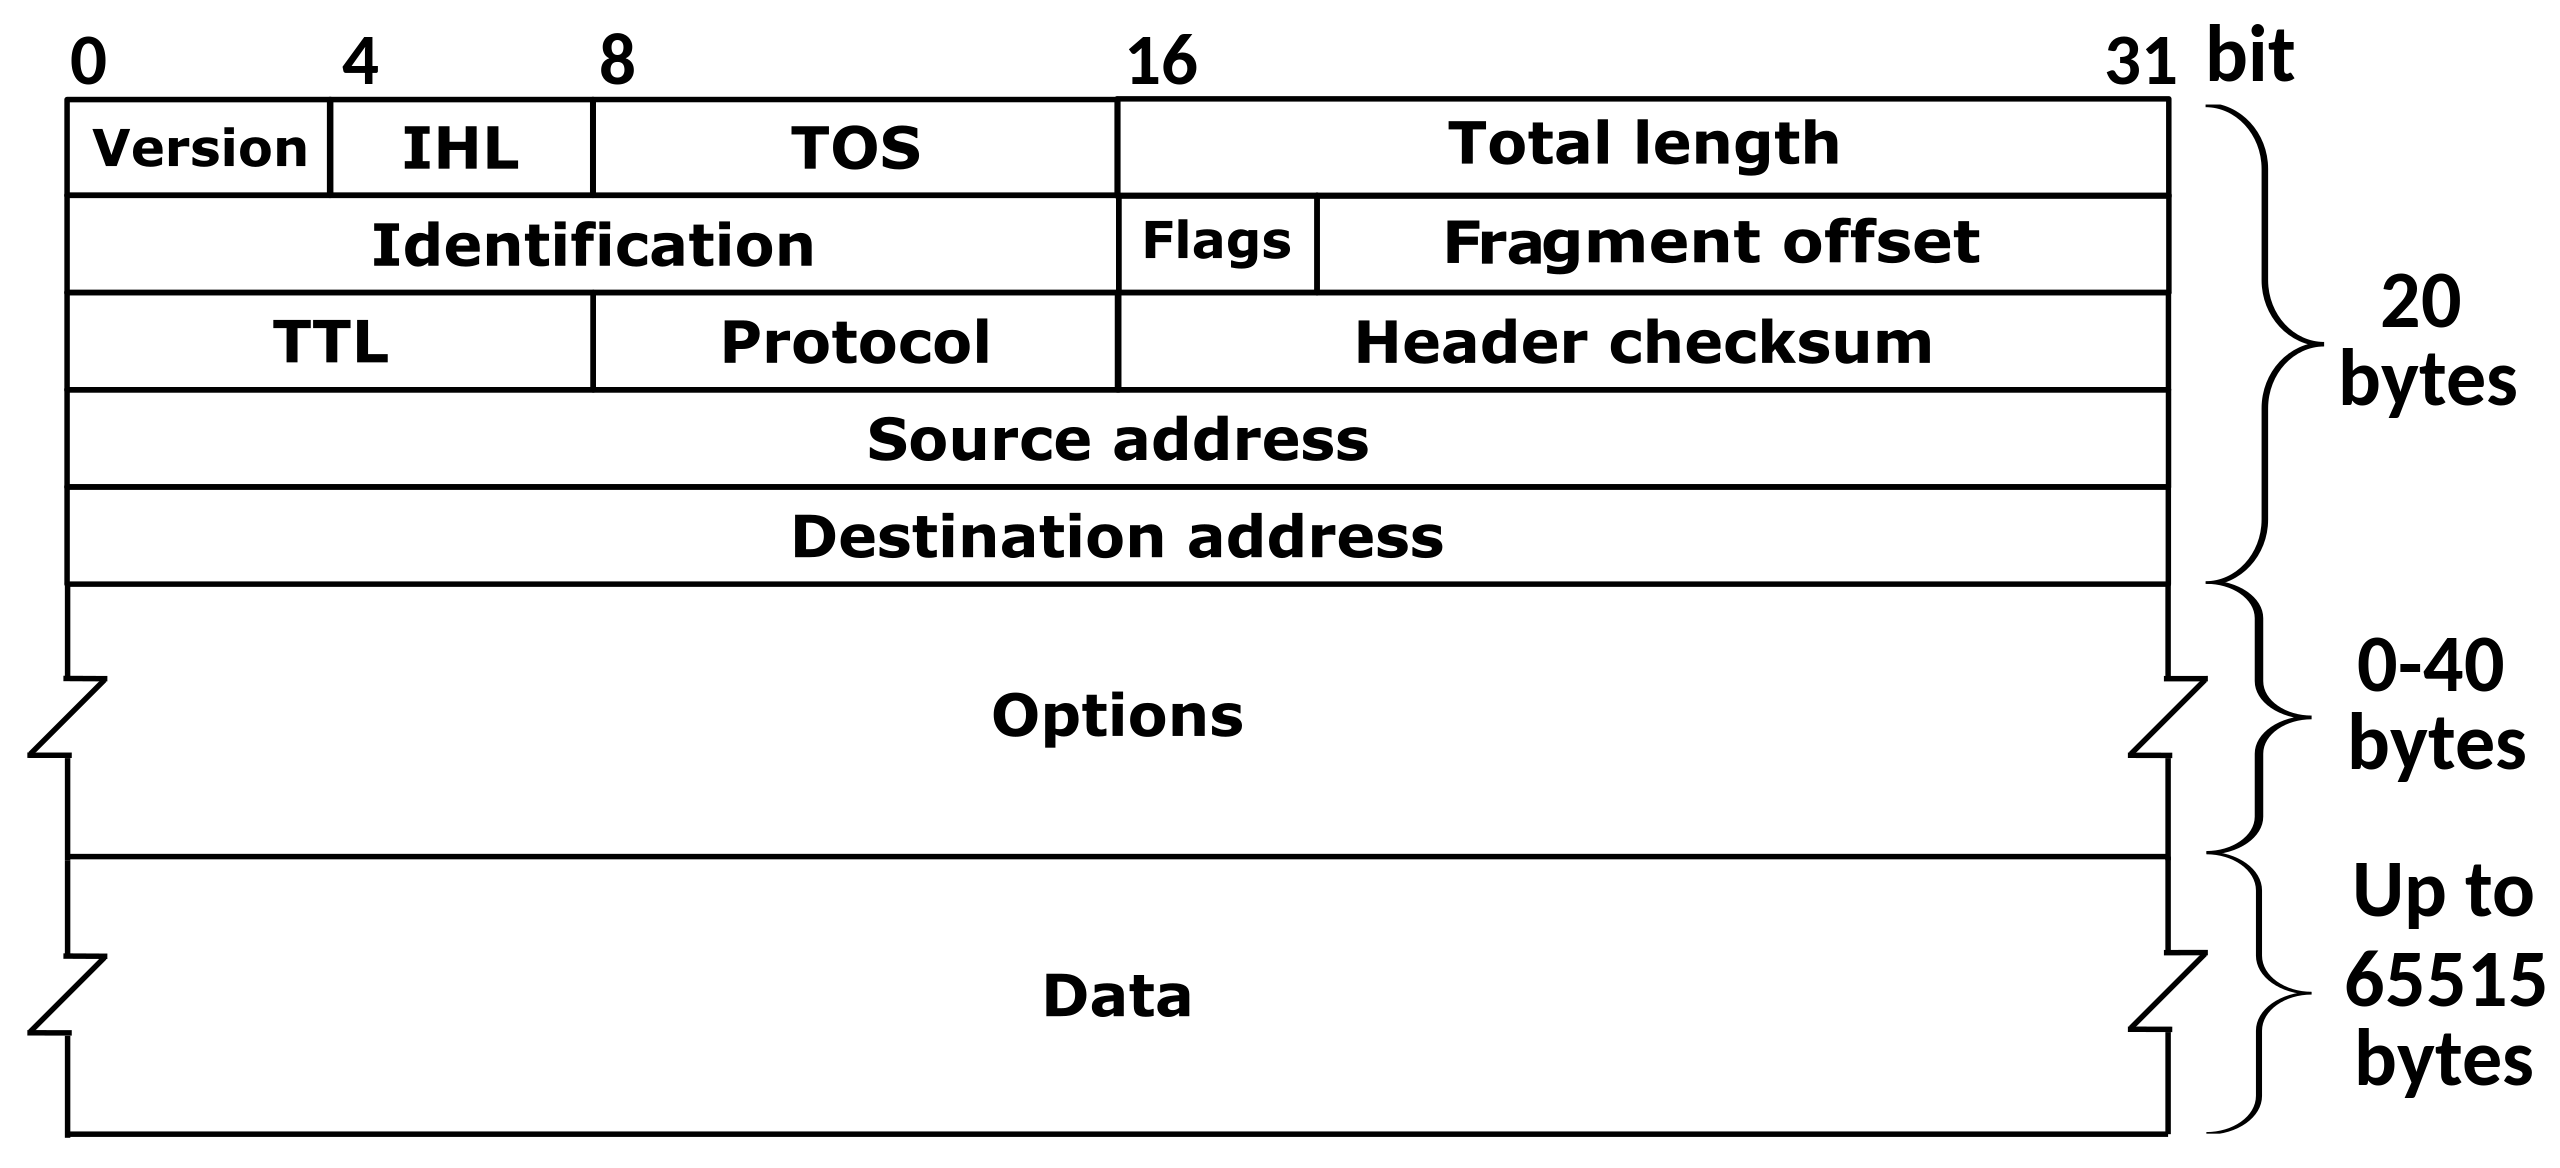
\includegraphics[width=\textwidth]{images/ipv4_frame.png}
\end{figure}
